% Case-C cross-axis translational-stiffness comparison. Entry-angle ranges are
% the achieved pose-based conditions across the three stiffness settings.
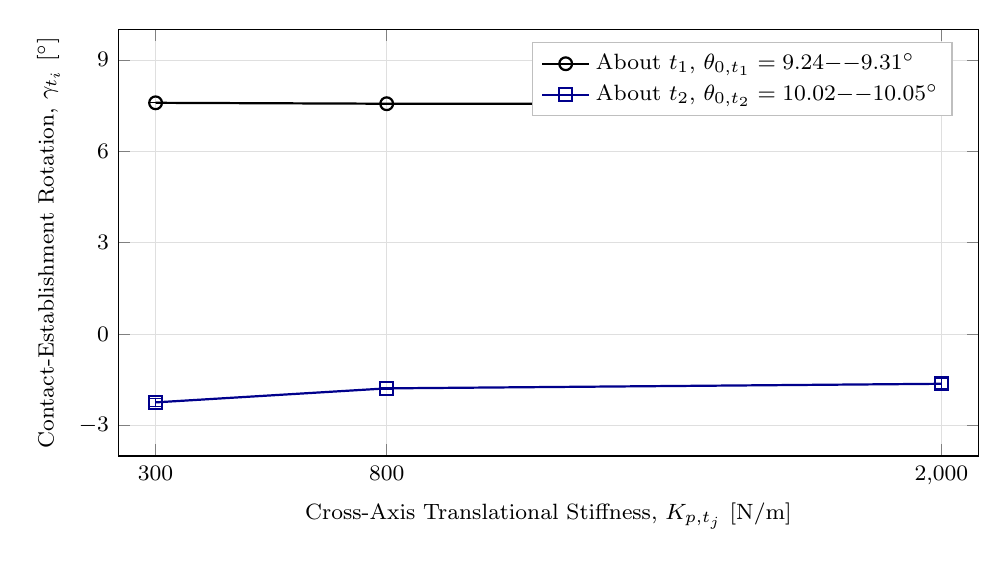
\begin{tikzpicture}
\begin{axis}[
    width=12.5cm, height=7.0cm,
    xmin=220, xmax=2080, ymin=-4, ymax=10,
    xtick={300,800,2000},
    ytick={-3,0,3,6,9},
    grid=major,
    grid style={gray!25, very thin},
    tick label style={font=\footnotesize},
    label style={font=\footnotesize},
    xlabel={Cross-Axis Translational Stiffness, \(K_{p,t_j}\) [N/m]},
    ylabel={Contact-Establishment Rotation, \(\gamma_{t_i}\) [\(^\circ\)]},
    legend style={font=\footnotesize, draw=gray!50, fill=white,
                  cells={anchor=west}},
    legend pos=north east,
    every axis plot/.append style={thick, mark size=2.3pt},
  ]
\addplot[black, mark=o, error bars/.cd, y dir=both, y explicit] coordinates {
  (300,7.59) +- (0,0.00) (800,7.56) +- (0,0.02) (2000,7.57) +- (0,0.01)};
\addlegendentry{About \(t_1\), \(\theta_{0,t_1}=9.24\text{--}9.31^\circ\)}
\addplot[blue!55!black, mark=square, error bars/.cd, y dir=both, y explicit] coordinates {
  (300,-2.24) +- (0,0.14) (800,-1.78) +- (0,0.03) (2000,-1.63) +- (0,0.17)};
\addlegendentry{About \(t_2\), \(\theta_{0,t_2}=10.02\text{--}10.05^\circ\)}
\end{axis}
\end{tikzpicture}
